\chapter{Impact on stakeholders and markets, strategic aspects}

This section starts by analysing an hipotetical situation. Let's supose that we have been hired as by a company with certain business, and we are taken into account as decision making advisors in the area of technology. The company has already made a decision about releasing their key software product under Apache or GPL license, and there is a new meeting to decide which license to choose? And more specifically: \textbf{Which license will attract more companies to collaborate in our business?}\\

We recall that the Apache license type can be classified as permissive, while a GPL as copyleft, each with its own implications. \\

The debate at class started with different approaches, some were inclined to the GPL because it ensured the continuity of the project under the same trend, others by Apache because commercial companies in general have less resistance to such licenses, and others ultimately could not come to any conclusion. Eventually all converged to that there is no formula with calculated results, the choice of a FLOSS license type usually depends on at least the following premises:

\begin{itemize}
\item Desired goal to be obtained with the product
\item Niche market to which the product is intended
\item Presence of the company in the current market
\item Preliminary study of the current market and definition of the possible innovation
\item Among many others
\end{itemize}

Overall we can see that the decision making regarding to Free Software, is not far from other business areas and corresponding analysis, every FLOSS product deserves its specific considerations.

\section{Impact on companies using software and in the production fabric}


One thing is very clear when talking about the economic impact that a business strategy can produce, and it is to be focused from a purely practical point of view. In this sence we watched the video\footnote{http://www.parc.com/event/1092/open-for-business.html} of a lecture at PARC (Palo Alto Research Center) about \textquotedblleft Open for business: Building successful commerce around open source", whose presenter was M\aa rten Mickos, Eucalyptus Systems CEO and ex-CEO of MySQL AB, two successful OSS companies.\\

Some main ideas about the presentation are:

\begin{itemize}
\item A business presentation, not a technical one
\item Make a lot of money with open source is the main goal, because companies are the ones who finances developers and so on, if it requires closed source features or going to the enterprise market, it has to be done in order to sustain
\item For many people is tough talking about FLOSS and business at the same time, because there are mistaken concepts around these topics together
\item FLOSS a better method to produce software (goods), faster (communities), common interest into solve problems (developers), relies over internet (distribution), users are happy with it (customers), but difficult to sell it (companies)
\item When talking from a practical point of view, it important to differentiate FLOSS from philosophical issues involved
\item Forms of production and distribution are very important, and in this case on intangible assets
\item Maybe FLOSS works because there are people trying to solve their own personal problems over this model, so maybe there is no charity or voluntary at all
\item Important companies such as RedHat or Oracle have inverted lots of money on FLOSS and have shown it is a sustainable model
\item Now when talking about FLOSS, words like: serious, commercial and professional, show up
\item Some time ago vendors didn't care about FLOSS, but now customers are demanding it
\item Before quality of software was dictated only by proprietary software companies, but now with FLOSS the quality is in sight of all people
\item The core-business for a company, may be non-core for others, this is a good feature to take advantage of
\item Eventually a company that successfully penetrates with FLOSS a market that was proprietary, tends to enforce the rules
\item FLOSS success vs Commercial success graphic:
\begin{figure}[h]
\begin{center}
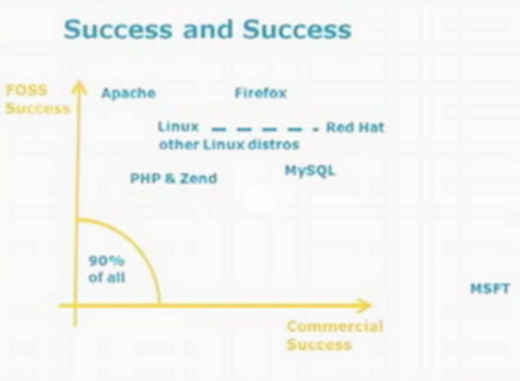
\includegraphics{success}
\caption{FLOSS success vs Commercial success}
\label{fig:success}
\end{center}
\end{figure}
\end{itemize}


\section{The Economic Motivation of Open Source Software: Stakeholder Perspectives}\label{Part II}

In working process... by Daniel G\'amez.\\

\section{Conclusions}\label{conclusions}
